\caulc 
%%%============= EX_1 =============%%%
\begin{ex}%[1D2N3-2]%[TDMZZ11]%[Mui Doan]
	Cho cấp số nhân $(u_n)$ có số hạng thứ hai bằng $1$ và số hạng thứ nhất bằng $2$. Công bội của $(u_n)$ bằng
	\choice
	{\True $\dfrac{1}{2}$}
	{$2$}
	{$3$}
	{$1$}
	\loigiai{
		Ta có công bội $q=\dfrac{u_2}{u_1}=\dfrac{1}{2}$.
	}
\end{ex}

%%%============= EX_2 =============%%%
\begin{ex}%[1D7N2-1]%[TDMZZ11]%[Mui Doan]
	Đạo hàm của hàm số $y=\ln(x+1)$ là
	\choice
	{\True $\dfrac{1}{x+1}$}
	{$x+1$}
	{$x-1$}
	{$\mathrm{e}^x$}
	\loigiai{
		Ta có $y'=\dfrac{1}{x+1}$.
	}
\end{ex}

%%%============= EX_3 =============%%%
\begin{ex}%[1D6N4-2]%[TDM21]%[Dự án TDM]
	Tập nghiệm của phương trình $3^{x^2-7} = 9$ là
	\choice
	{$\{\pm 2\}$}
	{\True $\{\pm 3\}$}
	{$\{\pm \sqrt{2}\}$}
	{$\{2\}$}
	\loigiai{
		Ta đưa hai vế của phương trình về cùng cơ số $3$:
		\[ 3^{x^2-7} = 9 \Leftrightarrow 3^{x^2-7} = 3^2. \]
		Cho hai số mũ bằng nhau, ta được:
		\[ x^2 - 7 = 2 \Leftrightarrow x^2 = 9 \Leftrightarrow \hoac{& x = 3 \\ & x = -3.} \]
		Vậy tập nghiệm của phương trình là $S = \{\pm 3\}$.
	}
\end{ex}

%%%============= EX_4 =============%%%
\begin{ex}%[1H8N7-1]%[TDMZZ11]%[Nguyễn Tấn Linh]
	Cho khối lăng trụ có diện tích đáy bằng $6$ và chiều cao bằng $4$. Thể tích của khối lăng trụ này bằng
	\choice
	{\True $24$}
	{$8$}
	{$36$}
	{$12$}
	\loigiai{
		Thể tích của khối lăng trụ đã cho là $V=B\cdot h=6\cdot 4=24$.
	}
\end{ex}

%%%============= EX_5 =============%%%
\begin{ex}%[1D3H2-5]%[TDMZZ11]%[Nguyễn Tấn Linh]
	Giới hạn $\lim\limits_{x\to 2}\dfrac{\sqrt{x^2+5}-3}{x-2}$ bằng
	\choice
	{$\dfrac{1}{3}$}
	{$2$}
	{$4$}
	{\True $\dfrac{2}{3}$}
	\loigiai{
		Ta có
		\begin{align*}
			\lim\limits_{x\to 2}\dfrac{\sqrt{x^2+5}-3}{x-2} &= \lim\limits_{x\to 2}\dfrac{x^2+5-9}{(x-2)\left(\sqrt{x^2+5}+3\right)}\\
			&= \lim\limits_{x\to 2}\dfrac{(x-2)(x+2)}{(x-2)\left(\sqrt{x^2+5}+3\right)}\\
			&= \lim\limits_{x\to 2}\dfrac{x+2}{\sqrt{x^2+5}+3}\\
			&= \dfrac{2}{3}.
		\end{align*}
	}
\end{ex}

%%%============= EX_6 =============%%%
\begin{ex}%[2D1N1-2]%[TDMZZ11]%[Bồ Văn Hậu]
	\immini[thm]{Cho bảng biến thiên của hàm số $f(x)$ như hình vẽ bên. Hỏi hàm số $f(x)$ nghịch biến trên khoảng nào, trong các khoảng dưới đây?}{
\begin{tikzpicture}[line join = round, line cap=round,>=stealth,font=\footnotesize,scale=0.75]	
			\tkzTabInit[lgt=1.2,espcl=2.5,deltacl=0.5]
			{$x$ /1,$f(x)$ /2}
			{$-\infty$, $-4$, $0$, $3$, $+\infty$}
			\tkzTabVar{-/$-\infty$,+/$1$,-/$-3$,+/ $1$,-/$-\infty$}
	\end{tikzpicture}}
	\choice
	{$(-\infty;-4)$}
	{\True $(-4;0)$}
	{$(0;3)$}
	{$(-3;1)$}
	\loigiai{
		Dựa vào bảng biến thiên của hàm số $f(x)$, ta thấy hàm số nghịch biến trên từng khoảng $(-4;0)$; $(3;+\infty)$.
	}
\end{ex}

%%%============= EX_7 =============%%%
\begin{ex}%[2D4N1-3]%[TDMZZ11]%[Bồ Văn Hậu]
	Cho hàm số $f(x)=2+\sin x$. Trong các khẳng định sau, khẳng định nào \textbf{đúng}?
	\choice
	{$\displaystyle\int\limits f(x) \mathrm{\,d}x=2x+\cos x+C$}
	{$\displaystyle\int\limits f(x) \mathrm{\,d}x= 2-\cos x+C$}
	{\True $\displaystyle\int\limits f(x) \mathrm{\,d}x=2x-\cos x+C$}
	{$\displaystyle\int\limits f(x) \mathrm{\,d}x=2+\cos x+C$}
	\loigiai{
		Ta có $\displaystyle\int\limits f(x) \mathrm{\,d}x = \displaystyle\int\limits \left(2 + \sin x\right) \mathrm{\,d}x = \displaystyle\int\limits 2 \mathrm{\,d}x + \displaystyle\int\limits \sin x \mathrm{\,d}x=2x-\cos x+C$.
	}
\end{ex}

%%%============= EX_8 =============%%%
\begin{ex}%[2H2N2-4]%[TDMZZ11]%[Lê Phúc]
	Trong không gian $Oxyz$, tích vô hướng của hai vectơ $\overrightarrow{u}=(1;0;3)$ và $\overrightarrow{v}=(-2;5;1)$ có giá trị bằng
	\choice
	{$-1$}
	{\True $1$}
	{$4$}
	{$2$}
	\loigiai{
		Ta có $\overrightarrow{u}\cdot \overrightarrow{v}=1\cdot (-2)+0\cdot 5+3\cdot 1=1$.
	}
\end{ex}

%%%============= EX_9 =============%%%
\begin{ex}%[2D1V1-4]%[TDMZZ11]%[Dự án TDM]
	\immini[thm]
	{
		Cho đồ thị hàm đa thức bậc năm $y=f(x)$ như hình vẽ. Hỏi phương trình $\sqrt{f(x)} \cdot \sqrt{f'(x)} = 0$ có tất cả bao nhiêu nghiệm thực phân biệt?
		\choice
		{\True $5$}
		{$6$}
		{$7$}
		{$4$}
	}
	{
		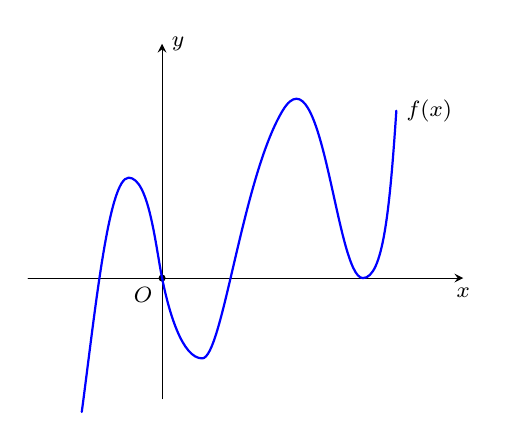
\begin{tikzpicture}[font=\footnotesize, line join=round, line cap=round, >=stealth, scale=0.85]
			% Vẽ hệ trục tọa độ
			\draw[->] (-2,0) -- (4.5,0) node[below] {$x$};
			\draw[->] (0,-1.8) -- (0,3.5) node[right] {$y$};
			\fill (0,0) circle (1.5pt) node[below left] {$O$};
			
			% Vẽ đồ thị hàm bậc 5 bằng Bezier curves
			\draw[thick, blue] (-1.2,-2)
			.. controls (-1,-0.5) and (-0.8,1.5) .. (-0.5,1.5)
			.. controls (-0.2,1.5) and (-0.1,0.5) .. (0,0)
			.. controls (0.1,-0.5) and (0.3,-1.2) .. (0.6,-1.2)
			.. controls (0.9,-1.2) and (1.2,1.5) .. (1.8,2.5)
			.. controls (2.4,3.5) and (2.6,0) .. (3,0)
			.. controls (3.3,0) and (3.4,1) .. (3.5,2.5) node[right, black] {$f(x)$};
		\end{tikzpicture}
	}
	\loigiai{
		Điều kiện xác định của phương trình: $\heva{& f(x) \ge 0 \\ & f'(x) \ge 0.}$ \hfill (*)
		
		Phương trình đã cho tương đương với:
		\[ \sqrt{f(x)} \cdot \sqrt{f'(x)} = 0 \Leftrightarrow \hoac{& f(x) = 0 \\ & f'(x) = 0.} \]
		
		\textbf{Trường hợp 1:} Giải phương trình $f(x) = 0$.\\
		Dựa vào sự tương giao của đồ thị $y=f(x)$ và trục hoành $y=0$, phương trình có $4$ nghiệm phân biệt (gọi hoành độ giao điểm từ trái sang phải lần lượt là $x_1, x_2, x_3, x_4$). Ta kiểm tra điều kiện $f'(x) \ge 0$ (nghĩa là kiểm tra tính đồng biến/nghịch biến tại các điểm đó):
		\begin{itemize}
			\item Tại nghiệm $x_1 < 0$: Đồ thị đang đi lên (hàm số đồng biến) nên $f'(x_1) > 0$. Suy ra $x_1$ thỏa mãn điều kiện (*).
			\item Tại nghiệm $x_2 = 0$: Đồ thị đang đi xuống (hàm số nghịch biến) nên $f'(0) < 0$. Suy ra $x_2=0$ bị loại do vi phạm điều kiện.
			\item Tại nghiệm $x_3 \in (0; x_4)$: Đồ thị đang đi lên (hàm số đồng biến) nên $f'(x_3) > 0$. Suy ra $x_3$ thỏa mãn điều kiện (*).
			\item Tại nghiệm $x_4 > 0$: Đây là điểm cực tiểu, đồ thị tiếp xúc với trục hoành nên $f'(x_4) = 0$. Suy ra $x_4$ thỏa mãn điều kiện (*).
		\end{itemize}
		Vậy từ phương trình $f(x) = 0$, ta thu được $\mathbf{3}$ nghiệm phân biệt thỏa mãn hệ điều kiện.
		
		\textbf{Trường hợp 2:} Giải phương trình $f'(x) = 0$.\\
		Nghiệm của phương trình $f'(x) = 0$ chính là hoành độ các điểm cực trị của hàm số. Dựa vào đồ thị, hàm số có $4$ điểm cực trị (gọi hoành độ lần lượt là $a, b, c, d$ từ trái sang phải). Ta kiểm tra điều kiện $f(x) \ge 0$ (kiểm tra dấu của tung độ điểm cực trị):
		\begin{itemize}
			\item Tại điểm cực đại $x = a < 0$: Tung độ cực đại $f(a) > 0$. Suy ra $x=a$ thỏa mãn điều kiện (*).
			\item Tại điểm cực tiểu $x = b \in (0; x_3)$: Tung độ cực tiểu $f(b) < 0$. Suy ra $x=b$ bị loại.
			\item Tại điểm cực đại $x = c \in (x_3; x_4)$: Tung độ cực đại $f(c) > 0$. Suy ra $x=c$ thỏa mãn điều kiện (*).
			\item Tại điểm cực tiểu $x = d = x_4$: Tung độ cực tiểu $f(d) = 0$. Nghiệm này thỏa mãn điều kiện (*) nhưng \textbf{bị trùng} với nghiệm $x_4$ đã đếm ở Trường hợp 1.
		\end{itemize}
		Vậy từ phương trình $f'(x) = 0$, ta thu được thêm $\mathbf{2}$ nghiệm phân biệt mới thỏa mãn.
		
		Tổng hợp cả hai trường hợp, phương trình đã cho có tất cả $3 + 2 = 5$ nghiệm thực phân biệt.
	}
\end{ex}

%%%============= EX_10 =============%%%
\begin{ex}%[2H5N1-2]%[TDMZZ11]%[Đình Nguyên]
	Trong không gian $Oxyz$, cho mặt phẳng $(\alpha)\colon 2x-3y+5=0$. Một vectơ pháp tuyến của mặt phẳng $(\alpha)$ có tọa độ là
	\choice
	{$(2;-3;5)$}
	{$(2;3;5)$}
	{\True $(2;-3;0)$}
	{$(2;-1;3)$}
	\loigiai{
		Mặt phẳng $(\alpha)\colon 2x-3y+5=0$ có một vectơ pháp tuyến là $\overrightarrow{n}=(2;-3;0)$.
	}
\end{ex}

%%%============= EX_11 =============%%%
\begin{ex}%[2H2H1-2]%[TDMZZ11]%[Huỳnh Quốc Đạt]
	\immini[thm]{Cho hình chóp đều $S. ABCD$. Nhận xét nào dưới đây là \textbf{sai}?
		\choice
		{$\overrightarrow{SA} + \overrightarrow{SC} = \overrightarrow{SB} + \overrightarrow{SD}$}
		{\True $\overrightarrow{SA} + \overrightarrow{SB} + \overrightarrow{SC} + \overrightarrow{SD} = \overrightarrow{0}$}
		{$\overrightarrow{AB} + \overrightarrow{AD} = \overrightarrow{AC}$}
		{$\overrightarrow{BA} + \overrightarrow{BC} = \overrightarrow{BD}$}}{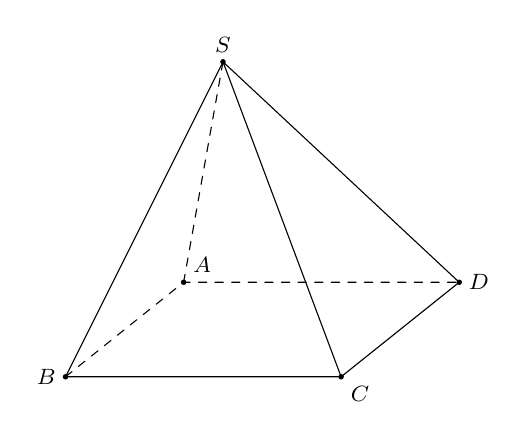
\begin{tikzpicture}[scale=1,font=\footnotesize,line join=round ,line cap=round,>=stealth]
			\draw[dashed] (2,4) coordinate (S) -- (1.5,1.2) coordinate (A) (0,0) coordinate (B) -- (A) -- (5,1.2) coordinate (D);
			\draw (S) -- (B) -- (3.5,0) coordinate (C) -- (D) -- (S) -- (C);
			\foreach \p/\pos/\lab in {
				{(A)}/above right/A, {(B)}/left/B, {(C)}/below right/C, {(D)}/right/D, {(S)}/above/S
			} {
				\fill \p circle (1pt);
				\node[\pos] at \p {$\lab$};
			}
	\end{tikzpicture}}
	\loigiai{
		Gọi $O$ là tâm của $ABCD$.\\
		Khi đó, ta có
		\[\overrightarrow{SA}+\overrightarrow{SB}+\overrightarrow{SC}+\overrightarrow{SD}=4\overrightarrow{SO}\neq \overrightarrow{0}.\]
	}
\end{ex}

%%%============= EX_12 =============%%%
\begin{ex}%[2D4V3-1]%[TDM21]%[Dự án TDM]
	Cho hình phẳng $(H)$ giới hạn bởi các đường $y=x\mathrm{e}^x$; $y=0$; $x=1$; $x=0$. Diện tích của hình phẳng $(H)$ bằng
	\choice
	{\True $1$}
	{$2$}
	{$e$}
	{$e-1$}
	\loigiai{
		Diện tích của hình phẳng $(H)$ được tính bởi công thức:
		\[ S = \displaystyle\int\limits_0^1 \left| x\mathrm{e}^x \right| \mathrm{\,d}x. \]
		Vì với mọi $x \in [0;1]$ ta luôn có $x \ge 0$ và $\mathrm{e}^x > 0$, suy ra $x\mathrm{e}^x \ge 0$. Do đó $\left| x\mathrm{e}^x \right| = x\mathrm{e}^x$.\\
		Ta có tích phân:
		\[ S = \displaystyle\int\limits_0^1 x\mathrm{e}^x \mathrm{\,d}x. \]
		Mặt khác, ta có đạo hàm:
		\[ \left[ (x-1)\mathrm{e}^x \right]' = (x-1)'\mathrm{e}^x + (x-1)\left(\mathrm{e}^x\right)' = 1 \cdot \mathrm{e}^x + (x-1)\mathrm{e}^x = \mathrm{e}^x + x\mathrm{e}^x - \mathrm{e}^x = x\mathrm{e}^x. \]
		Suy ra $F(x) = (x-1)\mathrm{e}^x$ là một nguyên hàm của hàm số $f(x) = x\mathrm{e}^x$.\\
		Khi đó:
		\allowdisplaybreaks
		\begin{align*}
			S &= \left. \left[ (x-1)\mathrm{e}^x \right] \right|_0^1 \\
			&= (1-1)\mathrm{e}^1 - (0-1)\mathrm{e}^0 \\
			&= 0 - (-1 \cdot 1) = 1.
		\end{align*}
		Vậy diện tích của hình phẳng $(H)$ bằng $1$.
	}
\end{ex}

\cauds 

%%%============= EX_13 =============%%%
\begin{ex}%[2D4H3-1]%[TDMZZ11]%[Dương Công Tạo]
	Trong mặt phẳng $Oxy$, cho hàm số $y = f(x) = 8x^3 -16x$. Gọi là $F(x)$ một nguyên hàm của hàm số $f(x)$ trên $\mathbb{R}$.
	\choiceTF
	{\True Đồ thị hàm số $y = f(x)$ có hai điểm cực trị đối xứng nhau qua gốc toạ độ}
	{Họ nguyên hàm của $f(x)$ là $F(x)+\left|C\right|$ với $C$ là một số thực}
	{\True Giá trị tích phân $\displaystyle\int\limits_0^2 F(x)\,\mathrm{d}x = -\dfrac{68}{15}$ và $F(0)=2$}
	{\True Khi đồ thị hàm số $y = F(x)$ đi qua gốc $O$ thì diện tích hình phẳng giới hạn bởi nó và trục hoành bằng $\dfrac{256}{15}$}
	\loigiai{
		\begin{itemchoice}
			\itemch Xét hàm số $y = f(x) = 8x^3 -16x$.\\
			Tập xác định $\mathscr{D}=\mathbb{R}$.\\
			Ta có \begin{itemize}
				\item $f(-x)=8\cdot(-x)^3-16\cdot(-x)=-8x^3+16x=-f(x)$.\quad(1)
				\item $f'(x)= 24x^2 -16$; $f'(x)=0\Leftrightarrow 24x^2 -16=0\Leftrightarrow x=\pm\dfrac{\sqrt{6}}{3}$.\\
				Bảng biến thiên
				\begin{center}
					
\begin{tikzpicture}[>=stealth]
						\tkzTabInit[nocadre=false,lgt=1.5,espcl=2,deltacl=0.6]{$x$/.7 ,$f'(x)$/.7,$f(x)$/2}
						{$-\infty$ , $-\tfrac{\sqrt{6}}{3}$ , $\tfrac{\sqrt{6}}{3}$ , $+\infty$}
						\tkzTabLine{ , + , $0$ , - , $0$ , + , }
						\tkzTabVar{-/$-\infty$ , +/$\dfrac{32\sqrt{6}}{9}$ , -/$-\dfrac{32\sqrt{6}}{9}$ , +/$+\infty$}
					\end{tikzpicture}
				\end{center}
				\noindent Dựa vào bảng biến thiên, ta thấy đồ thị hàm số có hai điểm cực trị.\quad(2)
			\end{itemize} 
			Từ (1) và (2) suy ra hai điểm cực trị này đối xứng nhau qua điểm $O$.
			\itemch Họ nguyên hàm của $f(x)$ là $F(x)+C$ với $C$ là một số thực tuỳ ý.
			\itemch Ta có $F(x)=\displaystyle\int \left(8x^3-16x\right)\mathrm{\,d}x =2x^4-8x^2+C$.\\
			Mà $F(0)=2$ nên $C=2$. Suy ra $F(x)=2x^4-8x^2+2$.\\
			Khi đó $\displaystyle\int\limits_0^2F(x)\mathrm{\,d}x=\displaystyle\int\limits_0^2\left(2x^4-8x^2+2\right)\mathrm{\,d}x=-\dfrac{68}{15}$.
			\itemch Khi đồ thị hàm số $y=F(x)$ đi qua gốc toạ độ thì $F(0)=0\Leftrightarrow C=0$. Suy ra $F(x)=2x^4-8x^2$.\\
			Xét phương trình $2x^4-8x^2=0\Leftrightarrow\hoac{&x=0\\&x=\pm 2.}$\\
			Khi đó, diện tích hình phẳng giới hạn bởi nó và trục hoành là \[S=\displaystyle\int\limits_{-2}^{2}\left|2x^4-8x^2\right|\mathrm{\,d}x=\dfrac{256}{15}.\]
		\end{itemchoice}
	}
\end{ex}

%%%============= EX_14 =============%%%
\begin{ex}%[2D6H1-2]%[TDMZZ11]%[Văn Minh Thoại]
	Xét một phép thử với hai biến cố $A$, $B$ thoả mãn $\mathrm{P}(A)=\dfrac{4}{5}$, $\mathrm{P}(B)=\dfrac{3}{5}$, $\mathrm{P}(A\cup B)=\dfrac{9}{10}$. 
	\choiceTF
	{\True $\mathrm{P}(A\cap B)=0{,}5$}
	{\True $\mathrm{P}(B\mid A)=0{,}625$}
	{\True $\mathrm{P}\left(B\mid\overline{A}\right)=0{,}5$}
	{\True $\mathrm{P}(A\mid A\cup B)=\dfrac{8}{9}$}
	\loigiai{
		Ta có $\mathrm{P}(A)=\dfrac{4}{5}=0{,}8$; $\mathrm{P}(B)=\dfrac{3}{5}=0{,}6$; $\mathrm{P}(A\cup B)=\dfrac{9}{10}=0{,}9$.
		\begin{itemchoice}
			\itemch  Ta có $\mathrm{P}(A\cup B)=\mathrm{P}(A)+\mathrm{P}(B)-\mathrm{P}(A\cap B)\Rightarrow \mathrm{P}(A\cap B)=\mathrm{P}(A)+\mathrm{P}(B)-\mathrm{P}(A\cup B)=0{,}8+0{,}6-0{,}9=0{,}5$.
			\itemch Theo công thức xác suất có điều kiện, ta có $\mathrm{P}(B\mid A)=\dfrac{\mathrm{P}(A\cap B)}{\mathrm{P}(A)}=\dfrac{0{,}5}{0{,}8}=0{,}625$.
			\itemch Ta có $\mathrm{P}\left(B\mid\overline{A}\right)=\dfrac{\mathrm{P}\left(B\cap\overline{A}\right)}{\mathrm{P}\left(\overline{A}\right)}=\dfrac{\mathrm{P}(B)-\mathrm{P}(A\cap B)}{1-\mathrm{P}(A)}=\dfrac{0{,}6-0{,}5}{1-0{,}8}=\dfrac{0{,}1}{0{,}2}=0{,}5$.
			\itemch Ta có $\mathrm{P}(A\mid A\cup B)=\dfrac{\mathrm{P}\big(A\cap(A\cup B)\big)}{\mathrm{P}(A\cup B)}=\dfrac{\mathrm{P}(A)}{\mathrm{P}(A\cup B)}=\dfrac{\dfrac{4}{5}}{\dfrac{9}{10}}=\dfrac{8}{9}$.
		\end{itemchoice}
	}
\end{ex}

%%%============= EX_15 =============%%%
\begin{ex}%[2H5V2-8]%[TDMZZ11]%[Vũ Hồng Toàn]
	Trong không gian $Oxyz$ đơn vị dài trên mỗi trục bằng $40$\,cm, có một nguồn sáng điểm $S(4; -2; 3)$. Có một chiếc gương phẳng nằm trên mặt phẳng $\left(Oxy\right)$ và một bức tường nằm trên mặt phẳng $(\alpha) \colon y - 6 = 0$. Một tia sáng xuất phát từ điểm $S$, gặp gương phẳng tại điểm $I(0; 2; 0)$ thì tia sáng sẽ bị phản xạ đổi hướng (bật trở lại) tại $I$ và gặp bức tường tại điểm $K$. Gọi $In$ là tia vuông góc với $(Oxy)$ tại $I$ nằm ở cùng phía $S$ so với $(Oxy)$. Khi đó ta có $IK \subset \left(S, In\right)$ và có $\widehat{KIn} = \widehat{SIn}$.
	\choiceTF
	{\True $\cos \widehat{SIn} = \dfrac{3}{\sqrt{41}}$}
	{\True Phương trình tham số của đường thẳng $SI$ là $\heva{&x = 4t \\& y = 2 - 4t \\& z = 3t}$}
	{\True Điểm đối xứng với $S$ qua mặt phẳng $(Oxy)$ là $S'(4; -2; -3)$}
	{Độ dài đoạn $IK$ bằng $132$\,cm \textit{(tính theo đơn vị centimet và làm tròn kết quả đến hàng đơn vị)}}
	\loigiai{
		\begin{itemchoice}
			\itemch Ta có $S(4; -2; 3)$ và $I(0; 2; 0)$. Vectơ $\overrightarrow{IS} = (4; -4; 3) \Rightarrow \left|\overrightarrow{IS}\right| = \sqrt{4^2 + (-4)^2 + 3^2} = \sqrt{41}$.\\ 
			Tia $In$ vuông góc với mặt phẳng $(Oxy)$ và nằm cùng phía $S$ ($z_S = 3 > 0$) nên có vectơ chỉ phương $\overrightarrow{k} = (0; 0; 1)$.
			Khi đó
			\[\cos \widehat{SIn} = \dfrac{\left|\overrightarrow{IS} \cdot \overrightarrow{k}\right|}{\left|\overrightarrow{IS}\right| \cdot \left|\overrightarrow{k}\right|} = \dfrac{\left|4 \cdot 0 + (-4) \cdot 0 + 3 \cdot 1\right|}{\sqrt{41} \cdot 1} = \dfrac{3}{\sqrt{41}}.\]
			\itemch Đường thẳng $SI$ đi qua $I(0; 2; 0)$ và có vectơ chỉ phương $\overrightarrow{IS} = (4; -4; 3)$ nên có phương trình tham số là $\heva{&x = 4t \\& y = 2 - 4t \\& z = 3t.}$
			\itemch Điểm $S(4; -2; 3)$ đối xứng qua mặt phẳng $(Oxy)$ ($z = 0$) là $S'(4; -2; -3)$.
			\itemch Theo tính chất phản xạ, tia phản xạ $IK$ là tia đối của tia $IS'$, do đó $I$, $K$, $S'$ thẳng hàng. Đường thẳng $IK$ chính là đường thẳng $S'I$.\\ 
			Vectơ $\overrightarrow{IS'} = (4; -4; -3)$. Phương trình đường thẳng $S'I$ là $\heva{&x = 4t \\& y = 2 - 4t \\& z = -3t.}$\\ 
			Điểm $K$ là giao điểm của đường thẳng $S'I$ và mặt phẳng $(\alpha) \colon y = 6$.\\ 
			Thay vào phương trình đường thẳng ta được $2 - 4t = 6 \Rightarrow -4t = 4 \Rightarrow t = -1$.\\ 
			Tọa độ điểm $K$ là $K(-4; 6; 3)$.\\ 
			Độ dài đoạn $IK = \sqrt{(-4 - 0)^2 + (6 - 2)^2 + (3 - 0)^2} = \sqrt{16 + 16 + 9} = \sqrt{41}$ (đơn vị độ dài).\\ 
			Đổi sang đơn vị centimet $IK = 40 \cdot \sqrt{41} \approx 256$\,cm.
		\end{itemchoice}
	}
\end{ex}

%%%============= EX_16 =============%%%
\begin{ex}%[2D4V3-5]%[TDMZZ11]%[Hà Văn Hảo]
	Miền $(H)$ được giới hạn bởi các cạnh $BC$, $CD$ của hình chữ nhật và các cung phần tư của đường elip $(E)$ và đường tròn $(C)$. Biết $(C)$ có bán kính bằng $15$ cm với tâm là trung điểm của cạnh $AD$ và $(E)$ là elip có hai tiêu điểm $H$ và $K$ cách nhau $10\sqrt{5}$ cm. Tiến hành gắn hệ trục tọa độ $Oxy$ vào hình vuông, với gốc $O$ trùng với trung điểm của cạnh $BC$, trục $Ox$ hướng theo vectơ $\overrightarrow{BC}$, trục $Oy$ hướng theo vectơ $\overrightarrow{BA}$, đơn vị dài trên mỗi trục bằng $1$ cm.
	\begin{center}
		\begin{tikzpicture}[scale=0.2, >=stealth]
			\coordinate (B) at (-15, 0);
			\coordinate (C) at (15, 0);
			\coordinate (A) at (-15, 25);
			\coordinate (D) at (15, 25);
			\coordinate (O) at (0, 0);
			\coordinate (M) at (0, 25); 
			\coordinate (H) at (-11.18, 0);
			\coordinate (K) at (11.18, 0);
			\fill[pattern=north west lines, pattern color=gray!80] 
			(B) -- (C) -- (D) 
			arc (0:-90:15) -- (0,10) 
			plot[domain=0:-15, samples=50] (\x, {10*sqrt(1 - (\x/15)^2)}) -- cycle;
			\draw[red, thick] (A) -- (B) -- (C) -- (D) -- cycle;
			\draw[blue, very thick] plot[domain=-15:0, samples=100] (\x, {10*sqrt(1 - (\x/15)^2)});
			\node[blue] at (-8, 10) {$(E)$};
			\draw[blue, very thick] (0,10) arc (-90:0:15);
			\node[blue] at (9, 15) {$(C)$};
			\draw[dashed] (0,0) -- (0,25);
			\fill (0,10) circle (0.3); 
			\node at (0,26) {$30$};
			\fill (H) circle (0.3) node[below] {$H$};
			\fill (K) circle (0.3) node[below] {$K$};
			\draw[thick] (-13.5, -0.6) -- (-13, 0.6) (-13, -0.6) -- (-12.5, 0.6);
			\draw[thick] (13.5, -0.6) -- (14, 0.6) (13, -0.6) -- (13.5, 0.6);
			\draw[<->] (-11.18, -3) -- node[above] {$10\sqrt{5}$} (11.18, -3);
			\node at (A) [above left] {$A$};
			\node at (B) [below left] {$B$};
			\node at (C) [below right] {$C$};
			\node at (D) [above right] {$D$};
		\end{tikzpicture}
	\end{center}
	\choiceTF
	{\True $AB = 25$ cm}
	{\True Phương trình của cung tròn $(C)$ là $y = 25 - \sqrt{225 - x^2}$}
	{Diện tích của $(H)$ bằng $325$ cm$^2$ \textit{(làm tròn kết quả đến hàng đơn vị)}}
	{Một vật trang trí có dạng một khối tròn xoay được tạo thành khi miền $(H)$ quay quanh trục $BC$. Thể tích của vật thể này bằng $7\,823$ cm$^3$ \textit{(làm tròn kết quả đến hàng đơn vị)}}
	\loigiai{
		Gắn hệ trục tọa độ $Oxy$ như đề bài $O(0;0)$ là trung điểm $BC$. Khi đó $B(-15;0)$, $C(15;0)$.\\ 
		Vì $ABCD$ là hình chữ nhật nên $BC = 30$ cm.\\
		Tâm của đường tròn $(C)$ là trung điểm $I$ của $AD$. Do bán kính $R=15$, cung tròn đi qua $D$ và điểm trên trục $Oy$, nên $I(0; y_I)$.
		\begin{itemchoice}
			\itemch Đường elip $(E)$ có tiêu cự $2c = 10\sqrt{5} \Rightarrow c = 5\sqrt{5}$. \\
			Trục lớn nằm trên $BC$ nên $a = \dfrac{BC}{2} = 15$.\\
			Ta có $b^2 = a^2 - c^2 = 15^2 - (5\sqrt{5})^2 = 225 - 125 = 100 \Rightarrow b = 10$.\\
			Đỉnh trên của elip là $(0;10)$. Cung elip $(E)$ có phương trình $y = 10\sqrt{1 - \dfrac{x^2}{225}}$ với $x \in [-15; 0]$.\\
			Tại $x=0$, $y=10$. Điểm này cũng thuộc cung tròn $(C)$ vì tính liên tục của biên miền $(H)$.\\
			Với cung tròn $(C)$ tâm $I(0; y_I)$ bán kính $R=15$, tại $x=0$ thì $y = y_I - 15 = 10 \Rightarrow y_I = 25$.\\
			Vậy $A(-15; 25)$, $D(15; 25)$. Suy ra $AB = 25$ cm.
			\itemch Đường tròn $(C)$ có tâm $I(0;25)$ và bán kính $R=15$.\\
			Phương trình đường tròn $x^2 + (y-25)^2 = 15^2 \Rightarrow (y-25)^2 = 225 - x^2$.\\
			Vì cung tròn nằm phía dưới tâm $I$ nên $y - 25 = -\sqrt{225 - x^2} \Rightarrow y = 25 - \sqrt{225 - x^2}$.
			\itemch Diện tích miền $(H)$ được tính bởi
			\[S = \displaystyle\int\limits_{-15}^{0} 10\sqrt{1 - \dfrac{x^2}{225}}\mathrm{\,d}x + \displaystyle\int\limits_{0}^{15} \left( 25 - \sqrt{225 - x^2} \right)\mathrm{\,d}x = S_1 + S_2.\]
			Ta có
			\begin{itemize}
				\item $S_1 = \displaystyle\int\limits_{-15}^{0} \dfrac{10}{15}\sqrt{15^2 - x^2}\mathrm{\,d}x = \dfrac{75}{2} \pi = 37{,}5\pi$.
				\item $S_2 = \displaystyle\int\limits_{0}^{15} 25\mathrm{\,d}x - \displaystyle\int\limits_{0}^{15} \sqrt{15^2 - x^2}\mathrm{\,d}x = 375 - \dfrac{225}{4} \pi = 375 - 56{,}25\pi$.
			\end{itemize}
			Vậy $S = 37{,}5\pi + 375 - 56{,}25\pi = 375 - 18{,}75\pi \approx 316$ cm$^2$.
			\itemch Thể tích khối tròn xoay khi quay $(H)$ quanh trục $BC$ (trục $Ox$) được tính bởi
			\[V = \pi \displaystyle\int\limits_{-15}^{0} \left( 10\sqrt{1 - \dfrac{x^2}{225}} \right)^2\mathrm{\,d}x + \pi \displaystyle\int\limits_{0}^{15} \left( 25 - \sqrt{225 - x^2} \right)^2\mathrm{\,d}x = V_1 + V_2.\]
			Ta có
			\begin{itemize}
				\item $V_1 = \pi \displaystyle\int\limits_{-15}^{0} 100 \left( 1 - \dfrac{x^2}{225} \right)\mathrm{\,d}x = 100\pi \left. \left(x - \dfrac{x^3}{675}\right) \right|_{-15}^{0} = 100\pi \left(0 - (-15 + 5)\right) = 1\,000\pi$.
				\item $V_2 = \pi \displaystyle\int\limits_{0}^{15} \left( 850 - x^2 - 50\sqrt{225 - x^2} \right)\mathrm{\,d}x = \pi \displaystyle\int\limits_{0}^{15} \left( 850 - x^2 \right)\mathrm{\,d}x - 50\pi \displaystyle\int\limits_{0}^{15} \left( \sqrt{225 - x^2} \right)\mathrm{\,d}x$.\\
				Do đó $V_2 = 11\,625\pi -\dfrac{5\,625}{2}\pi^2$.
			\end{itemize}
			Vậy	$V = 1\,000\pi + 11\,625\pi - \dfrac{5\,625}{2}\pi^2 = 12\,625\pi - 2\,812{,}5\pi^2 \approx 11\,904$ cm$^3$.\\
		\end{itemchoice}
	}
\end{ex}

\caukq 
%%%============= EX_17 =============%%%
\begin{ex}%[2D1V3-6]%[TDMZZ11]%[Dự án TDM]
	Người ta dùng hai đoạn dây xích sắt $AC$ và $BD$ để giữ chắc thăng bằng nằm ngang cho khúc gỗ nặng $CD$ như hình vẽ. Biết khúc gỗ dài $3$ m và hai đầu dây $C$, $D$ đều cao so với mặt đất là $1$ m, hai đầu $CD$ có thể di chuyển dọc theo phương ngang. Nếu biết chi phí đoạn dây $AC$ là $0{,}2$ triệu VNĐ/$1$ m còn chi phí đoạn dây $BD$ là $0{,}1$ triệu VNĐ/$1$ m. Hãy xác định tổng chi phí nhỏ nhất tính theo đơn vị triệu VNĐ để dùng cho công việc trên \textit{(làm tròn kết quả đến hàng phần trăm)}?
	\begin{center}
		\begin{tikzpicture}[scale=0.7, >=stealth, line join=round, line cap=round, font=\footnotesize]
			\def\a{6} \def\b{4} \def\l{11} \def\h{1} \def\lg{3}
			\def\d{3}
			\path (0,0) coordinate (O)
			+(90:\a) coordinate (A)
			+(\d,\h) coordinate (C)
			+({\d+\lg},\h) coordinate (D)
			++(0:\l) coordinate (O')
			+(90:\b) coordinate (B)
			;
			\fill [top color=brown!80!black!90, bottom color=brown!80!black!90, middle color=brown!10] (C)++(-90:.18) arc (-90:-270:.07 and .18)--++(0:\lg) arc (90:-90:.07 and .18)--cycle;
			\fill [brown!100!black!100] (D) ellipse (.07 and .18);
			\draw [very thick, red] (O)--(A) (O')--(B);
			\draw [semithick, blue] (A)--(C) (B)--(D);
			\draw [very thick] (O)++(180:2)--($(O')+(0:2)$);
			%
			\draw [dash pattern=on 1.5pt off 1.5pt] (A)--++(180:.5) (B)--++(0:.5) (D)--++(0:.5) (O)--++(-90:.5) (C)--++(90:.7) (D)--++(90:.7) (O')--++(-90:.5);
			\draw [<->] (A)++(180:.5)--++(-90:\a) node [pos=.5, sloped, fill=white] {$\a$ m};
			\draw [<->] (B)++(0:.5)--++(-90:\b) node [pos=.5, sloped, fill=white] {$\b$ m};
			\draw [<->] (D)++(0:.5)--++(-90:\h) node [pos=.5, right] {$\h$ m};
			\draw [<->] (O)++(-90:.5)--++(0:\l) node [pos=.5, fill=white] {$\l$ m};
			\draw [<->] (C)++(90:.7)--++(0:\lg) node [pos=.5, fill=white] {$\lg$ m};
			\foreach \r in {1,3}{
				\fill ($(C)!\r/4!(D)+(-90:.18)$)--++(-.3,-.82)--++(.6,0)--cycle;
			}
			%
			\foreach \x/\y in {A/90, B/90, C/-90, D/-90}{
				\draw [fill=black] (\x) circle (1pt) ++(\y:0.4) node {$\x$};
			}
		\end{tikzpicture}
	\end{center}
	\par
	\shortans[0]{1,74}
	\loigiai{
		\begin{center}
			\begin{tikzpicture}[scale=0.7, >=stealth, line join=round, line cap=round, font=\footnotesize]
				\def\a{6} \def\b{4} \def\l{11} \def\h{1} \def\lg{3}
				\def\d{3}
				\path (0,0) coordinate (O)
				+(90:\a) coordinate (A)
				+(\d,\h) coordinate (C)
				+({\d+\lg},\h) coordinate (D)
				++(0:\l) coordinate (O')
				+(90:\b) coordinate (B)
				($(O)!(C)!(A)$) coordinate (H)
				($(O')!(D)!(B)$) coordinate (K)
				;
				\draw [line width=2pt] (C)--(D);
				\draw [very thick, red] (O)--(A) (O')--(B);
				\draw [semithick, blue] (A)--(C) (B)--(D);
				\draw [very thick] (O)++(180:2)--($(O')+(0:2)$);
				%
				\draw [dash pattern=on 1.5pt off 1.5pt] (A)--++(180:.5) (B)--++(0:.5) (D)--++(0:.5) (O)--++(-90:.5) (C)--++(90:.5) (D)--++(90:.5) (O')--++(-90:.5);
				\draw [<->] (A)++(180:.5)--++(-90:\a) node [pos=.5, sloped, fill=white] {$\a$ m};
				\draw [<->] (B)++(0:.5)--++(-90:\b) node [pos=.5, sloped, fill=white] {$\b$ m};
				\draw [<->] (D)++(0:.5)--++(-90:\h) node [pos=.5, right] {$\h$ m};
				\draw [<->] (O)++(-90:.5)--++(0:\l) node [pos=.5, fill=white] {$\l$ m};
				\draw [<->] (C)++(90:.5)--++(0:\lg) node [pos=.5, fill=white] {$\lg$ m};
				%
				\pic [draw, angle radius=0.2cm] {right angle=C--H--A};
				\pic [draw, angle radius=0.2cm] {right angle=B--K--D};
				\draw [<->] (C)--(H) node [pos=.5, fill=white] {$x$ (m)}
				(D)--(K) node [pos=.5, fill=white] {$8-x$ (m)};
				\foreach \x/\y in {A/90, B/90, C/-90, D/-90, H/-45, K/-135, O/-135, O'/-40}{
					\draw [fill=black] (\x) circle (1pt) ++(\y:0.5) node {$\x$};
				}
			\end{tikzpicture}
		\end{center}
		Gọi $H$ là hình chiếu vuông góc của $C$ trên $OA$, $K$ là hình chiếu vuông góc của $D$ trên $O'B$. \\
		Đặt $CH=x$ (m) với $0 \le x \le 8$. \\
		Ta có \\
		$OH=OK=1$ (m). \\
		$AH=OA-OH=5$ (m). \\
		$BK=O'B-O'K=3$ (m). \\
		$DK=OO'-CD-x=8-x$ (m). \\
		Các tam giác $AHC$ và $BKD$ lần lượt vuông tại $H$, $K$ nên \\ $AC=\sqrt{CH^2+AH^2}=\sqrt{x^2+25}$ (m). \\
		$BD=\sqrt{DK^2+BK^2}=\sqrt{(8-x)^2+9}=\sqrt{x^2-16x+73}$ (m). \\
		Tổng chi phí cho hai đoạn dây $AC$ và $BD$ là
		\[f(x)=0{,}2 \sqrt{x^2+25}+0{,}1 \sqrt{x^2-16x+73} \text{ (triệu VNĐ)}.\]
		Đạo hàm của hàm số $f(x)$ là
		\[f'(x)=\dfrac{0{,}2x}{\sqrt{x^2+25}}+\dfrac{0{,}1(x-8)}{\sqrt{x^2-16x+73}}.\]
		Cho $f'(x)=0 \Leftrightarrow 2x\sqrt{x^2-16x+73} = (8-x)\sqrt{x^2+25}$.
		\begin{align*}
			&\Rightarrow 4x^2(x^2 - 16x + 73) = (x^2 - 16x + 64)(x^2 + 25) \\
			&\Leftrightarrow 4x^4 - 64x^3 + 292x^2 = x^4 - 16x^3 + 89x^2 - 400x + 1600 \\
			&\Leftrightarrow 3x^4 - 48x^3 + 203x^2 + 400x - 1600 = 0.
		\end{align*}
		Phương trình trên có nghiệm duy nhất $x_0 \approx 2{,}449$ trên đoạn $[0;8]$. \\
		Ta có $f(0) = 1 + 0{,}1\sqrt{73} \approx 1{,}85$; $f(8) = 0{,}3 + 0{,}2\sqrt{89} \approx 2{,}19$; và $f(x_0) \approx 1{,}74$. \\
		Do đó $\min\limits_{[0;8]}f(x) \approx 1{,}74$. \\
		Vậy chi phí nhỏ nhất cần tìm xấp xỉ $1{,}74$ triệu VNĐ.
	}
\end{ex}

%%%============= EX_18 =============%%%
\begin{ex}%[2D4C3-5]%[TDMZZ11]%[Nguyễn Văn Sang]
	Cho một bình ban có dạng hình lăng trụ tứ giác đều với cạnh đáy bằng $60\text{ cm}$ và cạnh bên bằng $90\text{ cm}$ ban đầu đang đựng nước có khoảng cách từ mặt thoáng đến đáy bình đủ lớn. Khi ta thả một quả cầu X vào thì thấy mực nước trong bình dâng lên thêm $2\text{ cm}$, ta thả tiếp quả cầu Y vào thì thấy mực nước trong bình dâng lên thêm $5\text{ cm}$ nữa. Biết quả cầu Y có bán kính gấp đôi quả cầu X và phần ngập trong nước của cả hai quả cầu (khoảng cách tính từ điểm thấp nhất của mỗi quả cầu tới mặt thoáng của nước) là như nhau. Hãy tính theo đơn vị centimet bán kính của quả cầu X \textit{(làm tròn kết quả đến hàng đơn vị)}.
	\begin{center}
		\begin{tikzpicture}[scale=0.8, >=stealth, line join=round, line cap=round]
			% Tọa độ gốc cho bình lăng trụ
			\coordinate (A) at (0,0);
			\coordinate (B) at (6,-1.5);
			\coordinate (C) at (11,0.5);
			\coordinate (D) at (5,2);
			
			\def\H{7} % Chiều cao bình
			\def\h{3.5} % Chiều cao mực nước ban đầu
			
			\coordinate (A') at ($(A)+(0,\H)$);
			\coordinate (B') at ($(B)+(0,\H)$);
			\coordinate (C') at ($(C)+(0,\H)$);
			\coordinate (D') at ($(D)+(0,\H)$);
			
			\coordinate (Aw) at ($(A)+(0,\h)$);
			\coordinate (Bw) at ($(B)+(0,\h)$);
			\coordinate (Cw) at ($(C)+(0,\h)$);
			\coordinate (Dw) at ($(D)+(0,\h)$);
			
			% 1. Các cạnh khuất của bình
			\draw[thick, black!40, dashed] (A) -- (D) -- (C);
			\draw[thick, black!40, dashed] (D) -- (D');
			\draw[thick, blue!40, dashed] (Aw) -- (Dw) -- (Cw);
			\draw[thick, blue!40, dashed] (D) -- (Dw);
			
			% 2. Vẽ hai quả cầu hoàn chỉnh (Đóng vai trò làm phần chìm trong nước)
			% Quả cầu X (O_X = (3.3, 3.65), R=1.2) - Bị ngập đúng một nửa
			\shade[ball color=orange!80] (3.3, 3.65) circle (1.2);
			% Quả cầu Y (O_Y = (7.2, 4.85), R=2.4) - Bị ngập phần tư dưới cùng
			\shade[ball color=teal!70] (7.2, 4.85) circle (2.4);
			
			% 3. Thể tích nước (Đổ màu nguyên khối giúp loại bỏ hoàn toàn lỗi chồng lớp màu)
			\fill[cyan!20, opacity=0.45] (A) -- (B) -- (C) -- (Cw) -- (Dw) -- (Aw) -- cycle;
			
			% Vẽ lại các đường outline của mặt nước để tạo khối 3D
			\draw[thick, blue!60] (A) -- (Aw);
			\draw[thick, blue!60] (B) -- (Bw);
			\draw[thick, blue!60] (C) -- (Cw);
			\draw[thick, blue!70] (Aw) -- (Bw) -- (Cw);
			
			% 4. Dùng Clipping để vẽ đè phần quả cầu "nổi" lên trên mặt nước
			% Xử lý quả cầu X
			\begin{scope}
				% Cắt giữ lại phần không gian phía trên đường elip mặt nước
				\clip (3.3 + 1.2, 3.65) arc (0:-180:1.2 and 0.45) -- (3.3 - 1.2, 7) -- (3.3 + 1.2, 7) -- cycle;
				\shade[ball color=orange!80] (3.3, 3.65) circle (1.2);
			\end{scope}
			% Vẽ elip giao tuyến của X với mặt nước
			\draw[thick, blue!80!black, dashed] (3.3, 3.65) ellipse (1.2 and 0.45);
			
			% Xử lý quả cầu Y
			\begin{scope}
				% Cắt giữ lại phần không gian phía trên đường elip mặt nước của Y
				\clip (7.2 + 2.078, 3.65) arc (0:-180:2.078 and 0.78) -- (7.2 - 2.078, 8) -- (7.2 + 2.078, 8) -- cycle;
				\shade[ball color=teal!70] (7.2, 4.85) circle (2.4);
			\end{scope}
			% Vẽ elip giao tuyến của Y với mặt nước
			\draw[thick, blue!80!black, dashed] (7.2, 3.65) ellipse (2.078 and 0.78);
			
			% 5. Các cạnh thấy của bình lăng trụ ngoài cùng
			\draw[thick, black!80] (A) -- (B) -- (C);
			\draw[thick, black!80] (A) -- (A');
			\draw[thick, black!80] (B) -- (B');
			\draw[thick, black!80] (C) -- (C');
			\draw[thick, black!80] (A') -- (B') -- (C') -- (D') -- cycle;
			
			% 6. Chú thích và ghi kích thước
			\node[ orange!90!black] at (2.0, 5.0) {\text{ Cầu X}} ;
			\node[ teal!90!black] at (8.7, 7.5) {\text{ Cầu Y}};
			
			\draw[<->, >=latex] ($(A)+(0,-0.6)$) -- ($(B)+(0,-0.6)$) node[midway, below, sloped] {$60\text{ cm}$};
			\draw[<->, >=latex] ($(B)+(0.6,-0.3)$) -- ($(C)+(0.6,-0.3)$) node[midway, below, sloped] {$60\text{ cm}$};
			\draw[<->, >=latex] ($(C)+(0.8,0)$) -- ($(C')+(0.8,0)$) node[midway, above, sloped] {$90\text{ cm}$};
			
			% Ký hiệu độ sâu ngập (h) giống nhau cho cả 2 quả cầu
			\draw[<->, >=latex, red, thick] (7.2, 2.45) -- (7.2, 3.65) node[midway, right, fill=white, inner sep=1pt] {$h$};
			\draw[<->, >=latex, red, thick] (3.3, 2.45) -- (3.3, 3.65) node[midway, left, fill=white, inner sep=1pt] {$h$};
		\end{tikzpicture}
	\end{center}
	\par
	\shortans[0]{15}
	\loigiai{
		\textbf{Nhắc lại kiến thức và Phân tích mặt cắt 2D của bài toán}
		\begin{center}
			\begin{tikzpicture}[scale=1.2, >=stealth, line join=round, line cap=round]
				% Khối nước
				\fill[cyan!15] (-3, 0) rectangle (7, -1.5);
				% Quả cầu X (R=1, ngập h=1 -> Nửa chìm nửa nổi)
				\draw[thick, orange!90!black] (0, 0) circle (1);
				\fill[orange!30, opacity=0.8] (0, 0) circle (1);
				\fill[orange!80!black] (0, 0) circle (1.5pt) node[below right] {$O_X$};
				\draw[->, thick, orange!80!black] (0, 0) -- (0.707, 0.707) node[midway, above left] {$R$};
				\draw[<->, red, thick] (-1.3, -1) -- (-1.3, 0) node[midway, left] {$h$};
				\draw[dashed, black!60] (0,-1) -- (-1.3,-1);
				\node[orange!80!black, font=\bfseries] at (0, -1.8) {\text{Quả cầu X}};
				% Quả cầu Y (Bán kính 2R, cùng ngập h=1 -> Tâm cách mặt nước 1 khoảng R)
				\draw[thick, teal!90!black] (4, 1) circle (2);
				\fill[teal!30, opacity=0.8] (4, 1) circle (2);
				\fill[teal!80!black] (4, 1) circle (1.5pt) node[below right] {$O_Y$};
				\draw[->, thick, teal!80!black] (4, 1) -- (4+1.414, 1+1.414) node[midway, above left] {$2R$};
				\draw[<->, red, thick] (6.5, -1) -- (6.5, 0) node[midway, right] {$h$};
				\draw[dashed, black!60] (4,-1) -- (6.5,-1);
				\node[teal!80!black, font=\bfseries] at (4, -1.8) {\text{Quả cầu Y}};
				\draw[blue!60, thick, dashed] (-3, 0) -- (7, 0) node[above left, font=\footnotesize, text=blue!80!black] {Mặt thoáng nước};
			\end{tikzpicture}
		\end{center}
		
		\begin{itemize}
			\item Thể tích chỏm cầu (phần khối cầu ngập trong nước) có chiều cao $h$ và bán kính quả cầu $R$ được tính bằng công thức
			\[ \boxed{V = \dfrac{\pi h^2}{3}(3R - h)} \]
			\item Gọi $h$ là chiều cao phần ngập trong nước của cả hai quả cầu ($h > 0$).
			\item Gọi $R$ là bán kính quả cầu X. Theo giả thiết, bán kính quả cầu Y sẽ là $2R$.
		\end{itemize}
		\textbf{Lời Giải chi tiết}
		\begin{itemize}
			\item Diện tích mặt đáy của bình lăng trụ tứ giác đều là
			\[ S = 60 \times 60 = 3\,600 \text{ (cm}^2).\]
			\item Thể tích phần ngập nước của quả cầu X (bằng chính thể tích nước bị dời chỗ khi khối X chìm vào):
			\[ V_X = S \cdot \Delta h_X = 3\,600 \times 2 = 7\,200 \text{ (cm}^3).\]
			\item Tương tự, thể tích phần ngập nước của quả cầu Y (bằng thể tích nước dời chỗ do Y dâng thêm):
			\[ V_Y = S \cdot \Delta h_Y = 3\,600 \times 5 = 18\,000 \text{ (cm}^3).\]
			\item Lập tỉ số thể tích phần chìm trong nước của Y và X:
			\[ \dfrac{V_Y}{V_X} = \dfrac{18\,000}{7\,200} = \dfrac{5}{2}.\]
			\item Áp dụng công thức thể tích chỏm cầu, ta thiết lập được phương trình:
			\[ \dfrac{\dfrac{\pi h^2}{3}(6R - h)}{\dfrac{\pi h^2}{3}(3R - h)} = \dfrac{5}{2} \Leftrightarrow \dfrac{6R - h}{3R - h} = \dfrac{5}{2}.\]
			\item Giải phương trình tìm mối liên hệ giữa chiều cao phần ngập $h$ và bán kính $R$:
			\[ 2(6R - h) = 5(3R - h) \Leftrightarrow 12R - 2h = 15R - 5h \Leftrightarrow 3h = 3R \Leftrightarrow h = R.\]
			\item Thế $h = R$ vào phương trình tính thể tích phần chìm của X, ta được:
			\[ V_X = \dfrac{\pi R^2}{3}(3R - R) = \dfrac{2\pi R^3}{3}.\]
			\[ \Rightarrow \dfrac{2\pi R^3}{3} = 7\,200 \Rightarrow R^3 = \dfrac{10\,800}{\pi}.\]
			\item Lấy căn bậc ba hai vế, ta tìm được bán kính quả cầu X:
			\[ R = \sqrt[3]{\dfrac{10\,800}{\pi}} \approx 15 \text{ (cm)}.\]
		\end{itemize}
	}
\end{ex}

%%%============= EX_19 =============%%%
\begin{ex}%[2D6V2-3]%[TDMZZ11]%[Duong Xuan Loi]
	Hộp I có $13$ bi đỏ và $8$ bi xanh, hộp II ban đầu không chứa bi nào. Tiến hành gieo một con xúc xắc cân đối và đồng chất $3$ lần liên tiếp. Ở mỗi lần nếu số chấm thu được nhỏ hơn $3$ thì ta lấy $2$ bi đỏ từ hộp I sang hộp II, nếu số chấm lớn hơn $2$ thì ta lấy $2$ bi đỏ và $1$ bi xanh từ I sang II. Hãy tính xác suất để sau $3$ lần gieo xúc xắc hộp II có $2$ bi xanh, nếu hộp I có số bi đỏ không ít hơn số bi xanh \textit{(làm tròn kết quả đến hàng phần trăm)}?
	\begin{center}
		\begin{tikzpicture}[scale=.8,>=stealth,line join=round,line cap=round,every node/.style={font=\normalsize},declare function={br=0.43;}]
			\begin{scope}[shift={(0,0)}]
				\draw[fill=gray!20,draw=gray!40,line width=0.6pt] (-2.5,2.5) -- (2.5,2.5) -- (2.5,4.5) -- (-2.5,4.5) -- cycle;
				\draw[fill=gray!30,draw=gray!40,line width=0.6pt] (-3.5,0.5) -- (-2.5,2.5) -- (-2.5,4.5) -- (-3.5,0.8) -- cycle;
				\draw[fill=gray!10,draw=gray!40,line width=0.6pt] (3.5,0.5) -- (2.5,2.5) -- (2.5,4.5) -- (3.5,0.8) -- cycle;
				\draw[fill=gray!5,draw=gray!40,line width=0.6pt] (-3.5,0.5) -- (3.5,0.5) -- (2.5,2.5) -- (-2.5,2.5) -- cycle;
				\foreach \x in {-1.5,-0.5,0.5,1.5}{
					\shade[ball color=red] (\x,2.3) circle (br);
				}
				\foreach \x in {-2.0,-1.0,0.0,1.0,2.0}{
					\shade[ball color=red] (\x,1.9) circle (br);
				}
				\foreach \x in {-1.5,-0.5,0.5,1.5}{
					\shade[ball color=red] (\x,1.5) circle (br);
				}
				\foreach \x in {-2.0,-1.0,0.0,1.0}{
					\shade[ball color=blue] (\x,1.1) circle (br);
				}
				\foreach \x in {-1.5,-0.5,0.5,1.5}{
					\shade[ball color=blue] (\x,0.7) circle (br);
				}
				\draw[fill=gray!15,draw=gray!40,line width=0.6pt] (-3.5,0.5) -- (3.5,0.5) -- (3.5,0.8) -- (-3.5,0.8) -- cycle;
				\draw[fill=white,draw=gray!40,line width=0.6pt] (-3.7,-1.5) -- (3.7,-1.5) -- (3.7,0.6) -- (-3.7,0.6) -- cycle;
				\draw[fill=gray!10,draw=gray!40,line width=0.6pt] (-3.7,0.6) -- (3.7,0.6) -- (3.5,0.8) -- (-3.5,0.8) -- cycle;
				\draw[fill=gray!15,draw=gray!40,line width=0.6pt] (-3.7,0.6) -- (-2.7,4.7) -- (-2.5,4.5) -- (-3.5,0.8) -- cycle;
				\draw[fill=gray!15,draw=gray!40,line width=0.6pt] (3.7,0.6) -- (2.7,4.7) -- (2.5,4.5) -- (3.5,0.8) -- cycle;
				\draw[fill=gray!15,draw=gray!40,line width=0.6pt] (-2.7,4.7) -- (2.7,4.7) -- (2.5,4.5) -- (-2.5,4.5) -- cycle;
				\node[draw=gray!80,fill=gray!10,line width=0.6pt,align=center,text width=2.5cm,inner sep=4pt] at (0,-0.45) {\textbf{Hộp I} \\ 13 bi đỏ \\ 8 bi xanh};
			\end{scope}
			\begin{scope}[shift={(8,0)}]
				\draw[fill=gray!20,draw=gray!40,line width=0.6pt] (-2.5,2.5) -- (2.5,2.5) -- (2.5,4.5) -- (-2.5,4.5) -- cycle;
				\draw[fill=gray!30,draw=gray!40,line width=0.6pt] (-3.5,0.5) -- (-2.5,2.5) -- (-2.5,4.5) -- (-3.5,0.8) -- cycle;
				\draw[fill=gray!10,draw=gray!40,line width=0.6pt] (3.5,0.5) -- (2.5,2.5) -- (2.5,4.5) -- (3.5,0.8) -- cycle;
				\draw[fill=gray!5,draw=gray!40,line width=0.6pt] (-3.5,0.5) -- (3.5,0.5) -- (2.5,2.5) -- (-2.5,2.5) -- cycle;
				\draw[fill=gray!15,draw=gray!40,line width=0.6pt] (-3.5,0.5) -- (3.5,0.5) -- (3.5,0.8) -- (-3.5,0.8) -- cycle;
				\draw[fill=white,draw=gray!40,line width=0.6pt] (-3.7,-1.5) -- (3.7,-1.5) -- (3.7,0.6) -- (-3.7,0.6) -- cycle;
				\draw[fill=gray!10,draw=gray!40,line width=0.6pt] (-3.7,0.6) -- (3.7,0.6) -- (3.5,0.8) -- (-3.5,0.8) -- cycle;
				\draw[fill=gray!15,draw=gray!40,line width=0.6pt] (-3.7,0.6) -- (-2.7,4.7) -- (-2.5,4.5) -- (-3.5,0.8) -- cycle;
				\draw[fill=gray!15,draw=gray!40,line width=0.6pt] (3.7,0.6) -- (2.7,4.7) -- (2.5,4.5) -- (3.5,0.8) -- cycle;
				\draw[fill=gray!15,draw=gray!40,line width=0.6pt] (-2.7,4.7) -- (2.7,4.7) -- (2.5,4.5) -- (-2.5,4.5) -- cycle;
				\node[draw=gray!80,fill=gray!10,line width=0.6pt,align=center,text width=2.5cm,inner sep=4pt] at (0,-0.45) {\textbf{Hộp II}};
			\end{scope}
			\begin{scope}[shift={(13.5,0)},scale=1.4] % Tăng scale và dịch y một chút để cân đối
				\draw[fill=white!95!gray,draw=gray!40,rounded corners=3pt,line width=0.6pt] (-0.6,-0.6) rectangle (0.6,0.6);
				\draw[fill=white!90!gray,draw=gray!40,rounded corners=3pt,line width=0.6pt] (0.6,-0.6) -- (1.1,-0.1) -- (1.1,1.1) -- (0.6,0.6) -- cycle;
				\draw[fill=white!98!gray,draw=gray!40,rounded corners=3pt,line width=0.6pt] (-0.6,0.6) -- (0.6,0.6) -- (1.1,1.1) -- (-0.1,1.1) -- cycle;
				\fill[black] (-0.3,-0.3) circle (2.5pt);
				\fill[black] (0.3,0.3) circle (2.5pt);
				\fill[black] (0.25,0.85) circle (2pt); % Tâm
				\fill[black] (-0.15,0.75) circle (2pt); % Góc trái dưới
				\fill[black] (0.45,0.75) circle (2pt); % Góc phải dưới
				\fill[black] (0.05,0.95) circle (2pt); % Góc trái trên
				\fill[black] (0.65,0.95) circle (2pt); % Góc phải trên
				\fill[black] (0.75,-0.2) circle (2pt);
				\fill[black] (0.75,0.15) circle (2pt);
				\fill[black] (0.75,0.5) circle (2pt);
				\fill[black] (0.95,0.0) circle (2pt);
				\fill[black] (0.95,0.35) circle (2pt);
				\fill[black] (0.95,0.7) circle (2pt);
			\end{scope}
		\end{tikzpicture}
	\end{center}
	\par
	\shortans[0]{0,46}
	\loigiai{
		Gọi $A$ là biến cố gieo được mặt có số chấm nhỏ hơn $3$, ta có $\mathrm{P}(A) = \dfrac{2}{6} = \dfrac{1}{3}$.\\
		Gọi $B$ là biến cố gieo được mặt có số chấm lớn hơn $2$, ta có $\mathrm{P}(B) = \dfrac{4}{6} = \dfrac{2}{3}$.\\
		Gọi $k$ là số lần xuất hiện biến cố $B$ trong $3$ lần gieo xúc xắc ($k \in \{0; 1; 2; 3\}$).\\
		Sau $3$ lần gieo, số bi chuyển từ hộp I sang hộp II là $2(3-k)+2k=6$ bi đỏ và $0(3-k) + 1k = k$ bi xanh.\\
		Số bi còn lại trong hộp I sau $3$ lần gieo là $13-6=7$ bi đỏ và $8-k$ bi xanh.\\
		Gọi $E$ là biến cố \lq\lq sau $3$ lần gieo xúc xắc hộp II có $2$ bi xanh\rq\rq.\\
		Ta có hộp II có $2$ bi xanh khi và chỉ khi $k = 2$.\\
		Gọi $F$ là biến cố \lq\lq hộp I có số bi đỏ không ít hơn số bi xanh\rq\rq.\\
		Ta có số bi đỏ không ít hơn số bi xanh khi $7 \ge 8 - k \Rightarrow k \ge 1$.\\
		Xác suất xảy ra biến cố $F$ là $\mathrm{P}(F) = \mathrm{P}(k=1) + \mathrm{P}(k=2) + \mathrm{P}(k=3)$.\\
		Ta có $\mathrm{P}(F) = \mathrm{C}_3^1 \cdot \left(\dfrac{2}{3}\right)^1 \cdot \left(\dfrac{1}{3}\right)^2 + \mathrm{C}_3^2 \cdot \left(\dfrac{2}{3}\right)^2 \cdot \left(\dfrac{1}{3}\right)^1 + \mathrm{C}_3^3 \cdot \left(\dfrac{2}{3}\right)^3 \cdot \left(\dfrac{1}{3}\right)^0 = \dfrac{6}{27} + \dfrac{12}{27} + \dfrac{8}{27} = \dfrac{26}{27}$.\\
		Biến cố $E \cap F$ xảy ra khi $k=2$ (vì $k=2$ thỏa mãn $k \ge 1$).\\
		Xác suất xảy ra biến cố $E \cap F$ là $\mathrm{P}(E \cap F) = \mathrm{P}(k=2) = \mathrm{C}_3^2 \cdot \left(\dfrac{2}{3}\right)^2 \cdot \left(\dfrac{1}{3}\right)^1 = \dfrac{12}{27}$.\\
		Xác suất để sau $3$ lần gieo xúc xắc hộp II có $2$ bi xanh, biết hộp I có số bi đỏ không ít hơn số bi xanh là $\mathrm{P}(E\mid F) = \dfrac{\mathrm{P}(E \cap F)}{\mathrm{P}(F)} = \dfrac{\dfrac{12}{27}}{\dfrac{26}{27}} = \dfrac{12}{26} = \dfrac{6}{13}$.\\
		Làm tròn kết quả đến hàng phần trăm ta được $0{,}46$.
	}
\end{ex}

%%%============= EX_20 =============%%%
\begin{ex}%[1H8V6-2]%[TDMZZ11]%[Lê Hồ Quang Minh]
	Cho hình chóp $S.ABCD$ có đáy $ABCD$ là hình bình hành. Biết rằng $\mathrm{d}(B, AD)=6$, $\mathrm{d}(S, BC)=8$, $\mathrm{d}(SA, BC)=4$. Biết góc nhị diện tù. Hãy tính theo đơn vị độ số đo góc nhị diện $\left[S, BC, D\right]$ \textit{(làm tròn kết quả đến hàng đơn vị)}?
	\par
	\shortans[0]{108}
	\loigiai{
		\immini{Gọi
			\begin{itemize}
				\item $K$ là hình chiếu của $S$ trên $BC$.
				\item $N$ và $P$ lần lượt là hình chiếu của $K$ trên $AD$ và $SN$.
				\item $H$ là hình chiếu của $S$ trên $NK$.
			\end{itemize}
			Theo giả thiết ta có
			\begin{itemize}
				\item $\mathrm{d}(B, AD)=6 \Rightarrow NK = 6$ (Vì $BC \parallel AD$).
				\item $\mathrm{d}(S, BC)=8 \Rightarrow SK = 8$.
			\end{itemize}
		}
		{\begin{tikzpicture}[scale=0.7, font=\footnotesize,line join=round, line cap=round, >=stealth]
				\path 
				(0,0) coordinate (A)
				++(-160:4) coordinate (D)
				++(0:4.5) coordinate (C)
				($(A)+(C)-(D)$) coordinate (B)
				($(A)+(1,4)$) coordinate (S)
				($(B)!0.6!(C)$) coordinate (K)
				($(A)!0.4!(D)$) coordinate (N)
				($(S)!0.6!(N)$) coordinate (P)
				($(K)!0.5!(N)$) coordinate (H)
				;
				\foreach \i in{B,C,D}{\draw (S)--(\i);};
				\draw (B)--(C)--(D) (S)--(K);
				\draw[dashed] (S)--(A)--(B) (A)--(D) (P)--(K)--(N)--(S)--(H);
				\pic[draw,angle eccentricity=1.8,angle radius=2mm]{right angle=S--K--B} pic[draw,angle eccentricity=1.8,angle radius=2mm]{right angle=K--N--A} pic[draw,angle eccentricity=1.8,angle radius=2mm]{right angle=K--P--S}
				pic[draw,angle eccentricity=1.8,angle radius=2mm]{right angle=N--K--C} pic[draw,angle eccentricity=1.8,angle radius=2mm]{right angle=S--H--K};
				\foreach \i/\g in {A/-90,D/-90,C/-90,B/-90,S/90,K/-30,N/150,P/180,H/-90}
				\fill[black] (\i) circle(1pt)+(\g:3mm)node[scale=1]{$\i$};
		\end{tikzpicture}}
		Ta có $BC \parallel AD \subset (SAD) \Rightarrow BC \parallel (SAD) \Rightarrow \mathrm{d}(SA, BC) = \mathrm{d}(K;(SAD)) = 4$.\\
		Vì $\heva{&BC \perp SK\\&BC \perp NK}$ nên $BC \perp (SNK)$.\\
		Mà $BC \parallel AD$ nên $AD \perp (SNK)$ $\Rightarrow (SAD) \perp (SNK)$.\\
		Lại có $(SAD) \cap (SNK) = SN$ và $KP \perp SN$.\\
		Suy ra $KP \perp (SAD)$, hay $\mathrm{d}(K;(SAD)) = KP = 4$.\\
		Vì $\heva{&SK \perp BC\\&NK \perp BC}$ nên $[S,BC,D] = [S,BC,N] = \widehat{SKN}$.\\
		Xét các tam giác vuông $SPK$ và $NPK$ có $\heva{&SP=\sqrt{SK^2-KP^2} = 4\sqrt{3}\\ &NP = \sqrt{NK^2 - KP^2} = 2\sqrt{5}} \Rightarrow SN = 2\sqrt{5} + 4\sqrt{3}$.\\
		Áp dụng định lí cosin trong tam giác $SNK$ có
		\[\cos \widehat{SKN} = \dfrac{SK^2 + NK^2 - SN^2}{2\cdot SK \cdot NK} = \dfrac{64+36-\left(2\sqrt{5}+4\sqrt{3}\right)^2}{2\cdot 8 \cdot 6} = \dfrac{2-\sqrt{15}}{6}.\]
		Suy ra $\widehat{SKN} \approx 108^\circ$.\\
		Vậy số đo góc nhị diện $[S,BC,D]$ xấp xỉ $108^\circ$.
	}
\end{ex}

%%%============= EX_21 =============%%%
\begin{ex}%[2H5V3-4]%[TDMZZ11]%[Nguyễn Đức Tuấn Anh]
	\immini[thm]{
		Trong không gian $Oxyz$ có đơn vị dài trên mỗi trục là $800$ km, bề mặt Trái Đất được mô tả bởi mặt cầu $x^2 + y^2 + z^2 = 64$, với mặt phẳng xích đạo là mặt phẳng $(Oxy)$. Một thiên thạch coi như hạt chuyển động trên một quỹ đạo được coi như đường thẳng có phương trình tham số $\heva{&x = 0 \\ &y = t \\ &z = -50 - 2t.}$
		Khi đã dự đoán được hướng bay người ta bố trí một trạm quan sát đặt tại một điểm trên đường Xích Đạo của Trái Đất sao cho khoảng cách ngắn nhất từ nó đến thiên thạch đạt nhỏ nhất bằng $b$ kilômet. Hãy tính $\dfrac{b}{100}$ \textit{(làm tròn kết quả đến hàng đơn vị)}?}{
		\begin{tikzpicture}[line cap=round, line join=round, >=stealth, font=\footnotesize]
			\shade[ball color=cyan!30!green!20] (0,0) circle (2);
			\draw[dashed, blue!60!black, thin] (2,0) arc (0:180:2 and 0.553);
			\draw[] (-2,0) -- (-2.5,0) (0,-2) -- (0,-2.5);
			\draw[->] (2,0) -- (2.75,0) node[right] {$y$};
			\draw[->] (0,2) -- (0,2.75) node[above] {$z$};
			\draw[thick, blue!70!black] (-2,0) arc (180:360:2 and 0.553);
			\draw[thick, blue!60!black] (0,0) circle (2);
			\draw[dashed] (0,0) -- (-0.8, -0.5) (-2,0)--(2,0) (0,-2)--(0,2);
			\draw[->] (-0.8, -0.5) -- (-2.4, -1.5) node[below right] {$x$};
			\fill (0,0) circle (1.5pt) node[above right] {$O$};
			\coordinate (M) at (-2,0);
			\coordinate (Da) at (-2, -3);
			\coordinate (Db) at (-5, 2);
			\coordinate (H) at ($(Da)!(M)!(Db)$);
			\draw[thick, red] (Da) -- (Db) node[right] {$d$};
			\coordinate (Meteor) at ($(Db)!1.02!(Da)$);
			\fill[orange!30] (Meteor) circle (3.5pt);
			\fill[orange] (Meteor) circle (2pt) node[right, font=\scriptsize, xshift=2pt] {Thiên thạch};
			\draw[dashed] (M) -- (H);
			\fill[red] (M) circle (2.5pt);
			\draw[->] (-3,1.5)node[above]{Trạm quan sát}--(M);
		\end{tikzpicture}
	}
	\par
	\shortans[0]{122}
	\loigiai{
		\begin{center}
			\begin{tikzpicture}[line cap=round, line join=round, >=stealth, font=\footnotesize]
				\shade[ball color=cyan!30, opacity=0.45] (0,0) circle (2);
				\draw[dashed, blue!60!black, thin] (2,0) arc (0:180:2 and 0.553);
				\draw[] (-2,0) -- (-2.5,0) (0,-2) -- (0,-2.5);
				\draw[->] (2,0) -- (2.75,0) node[right] {$y$};
				\draw[->] (0,2) -- (0,2.75) node[above] {$z$};
				\draw[thick, blue!70!black] (-2,0) arc (180:360:2 and 0.553);
				\draw[thick, blue!60!black] (0,0) circle (2);
				\draw[dashed] (0,0) -- (-0.8, -0.5) (-2,0)--(2,0) (0,-2)--(0,2);
				\draw[->] (-0.8, -0.5) -- (-2.4, -1.5) node[below right] {$x$};
				\fill (0,0) circle (1.5pt) node[above right] {$O$};
				\coordinate (M) at (-2,0);
				\coordinate (Da) at (-2, -3);
				\coordinate (Db) at (-5, 2);
				\coordinate (H) at ($(Da)!(M)!(Db)$);
				\draw[thick, red] (Da) -- (Db) node[right] {$d$};
				\coordinate (Meteor) at ($(Db)!1.02!(Da)$);
				\fill[orange!30] (Meteor) circle (3.5pt);
				\fill[orange] (Meteor) circle (2pt) node[right, font=\scriptsize, xshift=2pt] {Thiên thạch};
				\draw[blue] (M) -- (H)node[below left]{$N$};
				\fill[red] (M) circle (1.5pt)node[above left]{$M$};
			\end{tikzpicture}
		\end{center}
		Mặt phẳng xích đạo là mặt phẳng $(Oxy)$ có phương trình $z = 0$.\\
		Đường xích đạo của Trái Đất là giao tuyến của mặt cầu và mặt phẳng xích đạo, do đó nó là đường tròn $(C)$ nằm trong mặt phẳng $(Oxy)$ có phương trình $\heva{&x^2 + y^2 = 64 \\ &z=0.}$\\
		Gọi $M(x;y;0)$ là vị trí đặt trạm quan sát trên đường xích đạo, ta có $x^2 + y^2 = 64 \Rightarrow y \in [-8;8]$.\\
		Gọi $N(0;t;-50-2t)$ là một điểm thuộc quỹ đạo $\Delta$ của thiên thạch.
		Khi đó
		\begin{align*}
			MN^2 &= x^2 + (t - y)^2 + (-50 - 2t)^2 \\
			&= x^2 + y^2 + t^2 - 2yt + 4t^2 + 200t + 2\,500 \\
			&= 5t^2 + 2(100 - y)t + 2\,564.
		\end{align*}
		Khoảng cách ngắn nhất từ trạm quan sát $M$ đến thiên thạch là khoảng cách từ $M$ đến đường thẳng $\Delta$, đạt được khi $MN^2$ nhỏ nhất.\\
		Tam thức bậc hai $5t^2 + 2(100 - y)t + 2\,564$ có hệ số $a = 5 > 0$ nên đạt giá trị nhỏ nhất tại $t = -\dfrac{100 - y}{5}$.\\
		Khi đó
		\[\big(\mathrm{d}(M, \Delta)\big)^2 = 2\,564 - \dfrac{5(100 - y)^2}{25} = \dfrac{-y^2 + 200y + 2\,820}{5}. \]
		Để khoảng cách này đạt giá trị nhỏ nhất thì biểu thức $f(y) = -y^2 + 200y + 2\,820$ phải đạt giá trị nhỏ nhất trên đoạn $[-8;8]$.\\
		Xét hàm số $f(y) = -y^2 + 200y + 2\,820$ trên $[-8;8]$.\\
		Ta có $f'(y) = -2y + 200 > 0$, $\forall y \in [-8;8]$.\\
		Do đó hàm số $f(y)$ đồng biến trên đoạn $[-8;8]$.\\
		Suy ra $\min\limits_{[-8;8]} f(y) = f(-8) = -(-8)^2 + 200\cdot (-8) + 2\,820 = 1\,156$.\\
		Vậy giá trị nhỏ nhất của $\mathrm{d}(M, \Delta)$ là $\sqrt{\dfrac{1\,156}{5}}=\dfrac{34}{\sqrt{5}}$.\\
		Do đơn vị dài trên mỗi trục là $800$ km nên khoảng cách thực tế nhỏ nhất là
		\[ b = \dfrac{34}{\sqrt{5}} \cdot 800 = 5\,440\sqrt{5}. \]
		Vậy $\dfrac{b}{100} = 54{,}4\sqrt{5} \approx 122$.
	}
\end{ex}

%%%============= EX_22 =============%%%
\begin{ex}%[0D8C2-5]%[TDMZZ11]%[Dự án TDM]
	Dùng $5$ màu: đỏ, cam, vàng, lục, tím tô cho $12$ ô vuông nhỏ được bố trí như hình vẽ bên dưới.
	\begin{center}
		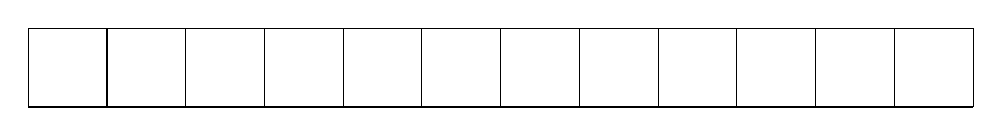
\begin{tikzpicture}[scale=1]
			\draw (0,0) grid (12,1);
		\end{tikzpicture}
	\end{center}
	Gọi $T$ là số cách tô màu thoả mãn đồng thời ba điều kiện sau:
	\begin{itemize}
		\item Mỗi ô vuông nhỏ được tô một màu.
		\item Có đúng ba ô vuông nhỏ được tô màu đỏ và giữa hai ô vuông màu đỏ có ít nhất $2$ ô vuông được tô màu khác với màu đỏ.
		\item Hai ô vuông cạnh nhau được tô màu khác nhau.
	\end{itemize}
	Biết rằng hai cách tô màu được gọi là khác nhau nếu tính từ trái sang phải có ít nhất một vị trí trong hai cách tô đó khác màu. Hãy tính $\dfrac{T}{1\,000}$ \textit{(làm tròn kết quả đến hàng đơn vị)}.
	\par
	\shortans[0]{2854}
	\loigiai{
		Cách tính số cách tô cho các ô không tô màu đỏ:
		\begin{itemize}
			\item Ô thứ nhất (đầu hàng) có $4$ cách. Các ô tiếp theo, nếu ô trước nó là đỏ thì ô đó có $4$ cách, nếu ô trước nó không phải đỏ thì nó có $3$ cách.
			\item Trong mọi trường hợp vị trí $3$ ô đỏ, ta luôn có: $4^3 \times 3^6$ cách tô cho các ô còn lại.
		\end{itemize}
		Giả sử các ô được đánh số từ $1$ đến $12$. Gọi vị trí $3$ ô màu đỏ lần lượt là $x_1, x_2, x_3$ ($1 \le x_1 < x_2 < x_3 \le 12$).\\
		Theo điều kiện, giữa hai ô đỏ có ít nhất $2$ ô khác màu đỏ, nên:
		$x_2 - x_1 \ge 3$ và $x_3 - x_2 \ge 3$.\\
		Đặt $y_1 = x_1$, $y_2 = x_2 - 2$, $y_3 = x_3 - 4$.\\
		Ta có $1 \le y_1 < y_2 < y_3 \le 12 - 4 = 8$.\\
		Ta xét các trường hợp sau:
		\begin{itemize}
			\item \textbf{TH1:} $1 = y_1 < y_2 < y_3 \le 7$.\\
			Số cách chọn vị trí cho $3$ ô đỏ là $\mathrm{C}_6^2 = 15$ cách.\\
			Theo cách tính ở trên, ta có số cách tô màu cho $9$ ô còn lại là $4^3\cdot 3^6$.\\
			Trường hợp này có $15\cdot 4^3\cdot 3^6$ cách.
			\item \textbf{TH2:} $2\le y_1 < y_2 < y_3=8$.\\
			Số cách chọn vị trí cho $3$ ô đỏ là $\mathrm{C}_6^2 = 15$ cách.\\
			Theo cách tính ở trên, ta có số cách tô màu cho $9$ ô còn lại là $4^3\cdot 3^6$.\\
			Trường hợp này có $15\cdot 4^3\cdot 3^6$ cách.
			\item \textbf{TH3:} $1=y_1 < y_2 < y_3=8$.\\
			Số cách chọn vị trí cho $3$ ô đỏ là $6$ cách (do $y_2 \in \{2;3;4;5;6;7\}$).\\
			Theo cách tính ở trên, ta có số cách tô màu cho $9$ ô còn lại là $4^2\cdot 3^7$.\\
			Trường hợp này có $6\cdot 4^2\cdot 3^7$ cách.
			\item \textbf{TH4:} $1<y_1 < y_2 < y_3<8$.\\
			Số cách chọn vị trí cho $3$ ô đỏ là $\mathrm{C}_6^3 = 20$ cách.\\
			Theo cách tính ở trên, ta có số cách tô màu cho $9$ ô còn lại là $4^4\cdot 3^5$.\\
			Trường hợp này có $20\cdot 4^4\cdot 3^5$ cách.
		\end{itemize}
		Tổng số cách là $T = 15\cdot 4^3\cdot 3^6+15\cdot 4^3\cdot 3^6+6\cdot 4^2\cdot 3^7+20\cdot 4^4\cdot 3^5= 2\,853\,792$.\\
		Suy ra $\dfrac{T}{1\,000} = \dfrac{2\,853\,792}{1\,000} = 2\,853{,}792\approx 2\,854$.
	}
\end{ex}
